\documentclass[11pt]{article} % article, report, or book
% \usepackage{geometry}                		% See geometry.pdf to learn the layout options. There are lots.
%\geometry{letterpaper}                   		% ... or a4paper or a5paper or ... 
\usepackage[margin=1.0in]{geometry}
%\usepackage[parfill]{parskip}    		% Activate to begin paragraphs with an empty line rather than an indent
\usepackage{graphicx}				% Use pdf, png, jpg, or eps§ with pdflatex; use eps in DVI mode
								% TeX will automatically convert eps --> pdf in pdflatex		
\usepackage{amsmath}
%\graphicspath{{/Users/lukebury/Documents/School/CU/ORCCA/}}
\usepackage{color}
\graphicspath{{../figures/}}

\usepackage[utf8]{inputenc} % allows for é
\usepackage{float} % allows for [H]

\newcommand{\paragraphtitle}[1]{\paragraph{#1}\mbox{}\\}
%=======================================================================================================
\title{APPM 5460 Final Project Proposal}
\author{Luke Bury \& Don Kuettel}
%=======================================================================================================
\begin{document}
\maketitle
%=======================================================================================================
\section*{Introduction}
This proposal aims to investigate homoclinic orbits in the dynamical system known as the Circular Restricted Three-Body Problem (CR3PB). The CR3PB, further described in the following section, is a classical astrodynamics problem that has been studied for over 200 years and contains a plethora of interesting dynamical phenomena, including homoclinic orbits. In mathematics, a homoclinic orbit is defined as a trajectory of a flow of a dynamical system which joins a saddle equilibrium point to itself. More precisely, a homoclinic orbit lies in the intersection of the stable manifold, $W^s(p)$, and the unstable manifold, $W^u(p)$, of an equilibrium. Figure \ref{f:homoclinic_example} shows an example of a simple, two-dimensional homoclinic orbit about the saddle equilibrium point $p$. As the figure shows, as time approaches either negative or positive infinity, the homoclinic orbit will approach $p$. 

\begin{figure}[H]
    \centering
    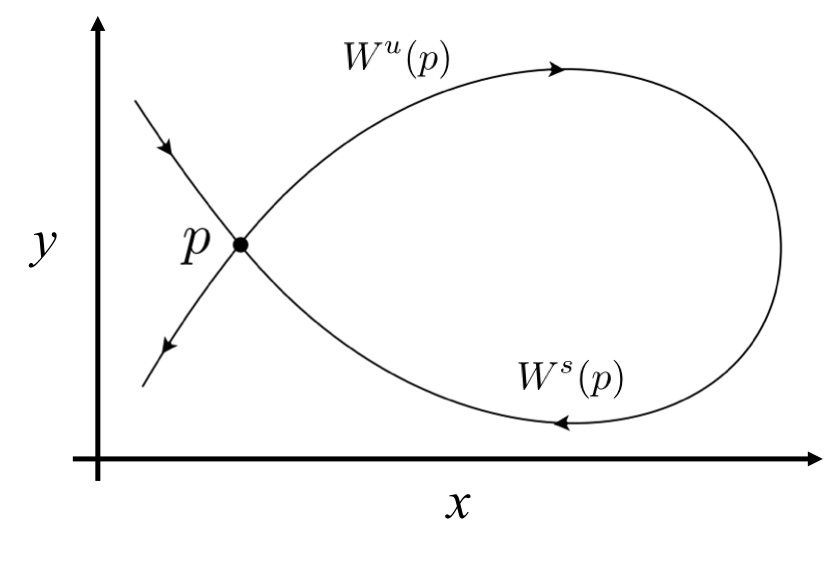
\includegraphics[width=4in]{homoclinic_orbit.png}
    \caption{This figure depicts a 2D homoclinic orbit.}
    \label{f:homoclinic_example}
\end{figure}

Homoclinic orbits, first discovered by Henri Poincar\'{e} in the 1885 Acta Mathematica competition sponsored by King Oscar II of Sweden, play an important role in the chaotic behavior of a dynamical system. Lying on the intersection between a stable and unstable manifold of the same equilibrium point, or orbit, the geometry of homoclinic orbits (i.e., the geometry of the manifold intersection) offers a way in which simple local information can be extrapolated to complicated global behavior. This proposal looks to study Poincar\'{e}'s work on homoclinic orbits and use that knowledge to find examples of homoclinic orbits in the CR3BP.


%-----------------------------------------------------------------------------------------
\section*{History of the Problem} % History / Lit Review
As documented by Andersson and Barrow-Green \cite{Andersson1994,BarrowGreen1994}, in 1885, Acta Mathematica announced a mathematics competition to the world. This competition, sponsored by King Oscar II of Sweden, encouraged interested parties to make an attempt at solving one of four selected problems. Henri Poincaré, a prominant mathematician of the time (who was largely favored to win the competition) attempted the first problem, which essentially asked for a solution to the troubling $n$-body problem. However, Poincaré instead decided to attempt a subset of the $n$-body problem known as the three-body problem, since it was the first order of the problem remaining unsolved. To further simplify his initial effort, Poincaré restricted the three-body system in a manner known today as the Circular Restricted Three-Body Problem (CR3BP), shown in Figure \ref{fig:CR3BP}. 

\begin{figure}[H]
\centering
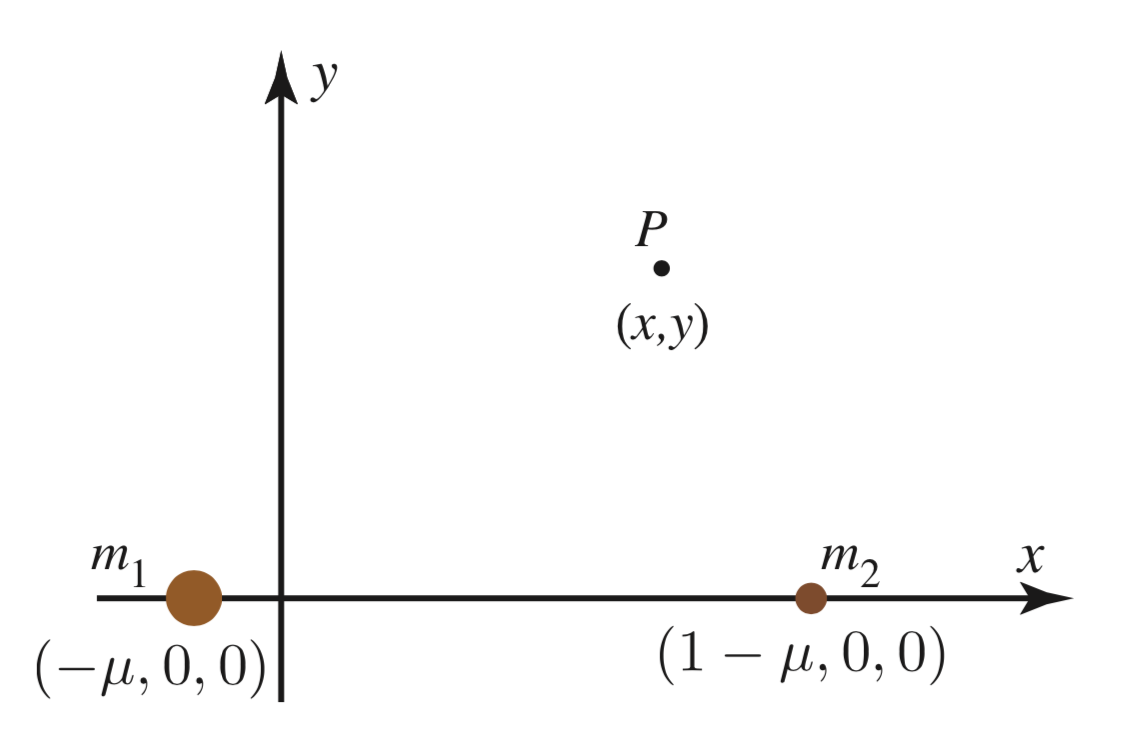
\includegraphics[width=3.75in]{CR3BP.png}\nonumber
\caption{Layout of Circular Restricted Three Body Problem \cite{KoonLoMarsdenRoss2011}}
\label{fig:CR3BP}
\end{figure}

In the CR3BP, the origin is set at the barycenter of the two main bodies in the system (e.g., the Earth \& Moon), and the frame rotates so these bodies remain stationary on the x-axis. The bodies are assumed to move in perfectly circular orbits and act as point masses from a gravitational perspective. The restricted problem is then to ascertain the motion of the third body whose mass is considered negligible. The system is typically normalized so that the masses of the two bodies sum to 1 ($m_1 = \mu,\; m_2 = 1-\mu$), the distance between the bodies is 1, and the gravitational constant G is equal to 1. Under these conditions, the equations of motion for the CR3BP are shown in Equations \ref{eomx}-\ref{eomz}:

\begin{align}
\ddot{x} &=  2\dot{y} + x - (1-\mu)\left(\dfrac{x+\mu}{R_1^3}\right) - \mu\left(\dfrac{x-1+\mu}{R_2^3}\right) \label{eomx}\\
\ddot{y} &= - 2\dot{x} + y\left(-\dfrac{1-\mu}{R_1^3} - \dfrac{\mu}{R_2^3} + 1\right) \label{eomy}\\
\ddot{z} &= z\left(-\dfrac{1 - \mu}{R_1^3} - \dfrac{\mu}{R_2^3}\right) \label{eomz}
\end{align}

Poincaré's submission to the competition consisted of the culmination of several strands of his work from the previous decade, which included geometrical and analytical theory, integral invariants, and periodic solutions to dynamical systems. Poincaré's applied these theories in an attempt to rigorously prove stability and find periodic solutions for the CR3BP. The competition judges immediately recognized the importance of Poincaré's submission and unanimoulsy crowned him the victor. However, around the time that his work was first being printed, a discussion with Lars Edvard Phragmén led to the discovery of an error within Poincaré's submission that held significant ramifications. The error was rooted in Poincaré's failing ``to take proper account of the exact geometric nature of a particular curve'' \cite{BarrowGreen1997}. In Theorem III of the paper's first, and flawed, edition, Poincaré claimed that a particular invariant curve was closed (Figure \ref{fig:curveIntersection1}(a,b)). He failed to consider that the curve could be self-intersecting (Figure \ref{fig:curveIntersection1}(c)). After realizing his mistake, Poincaré reworked his derivations to discover that the asymptotic surfaces are not closed but they intersect along infinitely many asymptotic trajectories. Ironically, this mistake cemented Poincaré's place among legendary mathematicians for his resulting discovery of \textit{doubly asymptotic}, or \textit{homoclinic}, points/orbits in the CR3PB and dynamical systems in general.  

\begin{figure}[H]
\centering
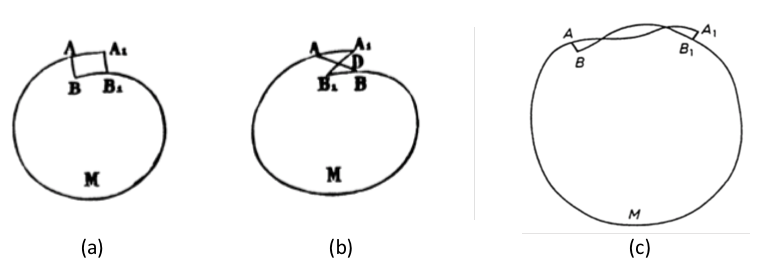
\includegraphics[width=5in]{curveIntersection1.png}\nonumber
\caption{(a) Diagrams of incorrectly closed invariant curves from the first edition of Poincaré's memoir. (b)Invariant curve with self intersection from Poincaré's corrected work \cite{BarrowGreen1997}}
\label{fig:curveIntersection1}
\end{figure}

%-----------------------------------------------------------------------------------------
\section*{Application of Poincaré's Results and Project Goals} 
Based on these famous results of Poincaré's work, this proposal looks to further investigate Poincaré's derivation of homoclinic orbits and to find several homoclinic orbits in the CR3BP. These two endeavors will constitute the two main topics of this project: (1) an analytical explanation of Poincaré's discovery of homoclinic orbits, and (2) a numerical study of homoclinic orbits in the CR3BP. The first part of this project is motivated by understanding the fundamental concepts of dynamical systems. By further investigating Poincaré's derivation of homoclinic orbits (i.e., the initial error in his competition submission), a deeper understanding of what homoclinic orbits represent for dynamical system can be reached. The second section of this project is then driven by the application of the theory. By investigating the intersections of the stable and unstable manifolds of periodic orbits around the equilibrium points in the CR3BP system, a subset of homoclinic trajectories can be systematically found in the CR3BP. This section of the project will focus on finding the equilibrium points (i.e., Lagrange points) within the CR3BP, developing a systematic approach to find periodic orbits, mapping the stable and unstable manifolds of several periodic orbits, and finally studying a Poincaré section of these manifolds to find homoclinic orbits of the periodic orbits. This proposal combines a study of Poincaré's discovery of homoclinic orbits with the application of the theory to create a mathematically interesting and challenging project. 

%=======================================================================================================
\newpage
\bibliographystyle{plain}
\bibliography{../bibliography/appm5460.bib}

\end{document}  